\section{Progress to Date}

\subsection{Overview}
\begin{itemize}
    \item A first draft of the \href{https://carrowmw.github.io/latex-documents/}{literature review} has been completed for the first research objective.
    \item The \href{https://github.com/carrowmw/phd-project}{codebase} has been largely built with regular commits on GitHub.
    \item A \href{}{dashboard} has been developed to demonstrate some of the functionality of the data quality measurement system.
    \item My research was \href{https://zenodo.org/records/10931950}{published} and presented at the \href{https://2024.gisruk.org/}{32\textsuperscript{nd} GISRUK Conference 2024}.
\end{itemize}

\subsection{CPD}
Up-skilling has been a major focus since January. Building scalable infrastructure requires knowledge of programming best practices beyond what was taught during the MRes. This includes understanding functional modularity, config-driven development, and object oriented programming paradigms, as well as specialised machine learning knowledge, for example, building Graph Neural Networks. I have completed a number of online, book-based and in-person courses to develop my programming and presentation skills, as well as attending all CDT organised events.

\textbf{External courses and training:}

\begin{itemize}
    \item \href{https://github.com/PacktPublishing/Hands-On-Graph-Neural-Networks-Using-Python}{Hands-On Graph Neural Networks Using Python}
    \item \href{https://app.datacamp.com/learn/courses/introduction-to-sql}{Introduction to SQL}
    \item \href{https://app.datacamp.com/learn/courses/hierarchical-and-recursive-queries-in-sql-server}{Hierarchical and Recursive Queries in SQL Server}
    \item \href{https://app.datacamp.com/learn/courses/object-oriented-programming-in-python}{Object-Oriented Programming in Python}
    \item \href{https://app.datacamp.com/learn/courses/introduction-to-llms-in-python}{Introduction to LLMs in Python}
    \item \href{https://app.datacamp.com/learn/courses/introduction-to-testing-in-python}{Introduction to Testing in Python}
    \item \href{https://app.datacamp.com/learn/courses/building-dashboards-with-dash-and-plotly}{Building Dashboards with Dash and Plotly}
    \item \href{https://app.datacamp.com/learn/courses/python-toolbox}{Python Toolbox}
    \item \href{https://app.datacamp.com/learn/courses/monitoring-machine-learning-concepts}{Monitoring Machine Learning Concepts}
\end{itemize}

\textbf{Newcastle University courses and workshops:}

\begin{itemize}
    \item Time Series Data - MAS8382
    \item The Introduction to Learning and Teaching (ILTHE)
    \item Building an Impactful Presentation: A Step-by-Step Guide
    \item Delivery Skills: Master the Art of Effective Presentations
    \item Storytelling for Researchers: Unleash the Power of Narrative
    \item Designing an Effective Research Poster
\end{itemize}

\subsection{Codebase and Dashboard}

The codebase which is primarily available here has been built with regular commits on GitHub. The codebase is structured to include the following components:

\begin{figure}[h]
    \caption{Top-level directory structure of the codebase.}
    \label{fig:top_level_tree}
    \begin{verbatim}
                    phd/
                    ├── apps/
                    ├── configs/
                    ├── data/
                    ├── logs/
                    ├── scripts/
                    ├── src/
                    │   ├── api/
                    │   ├── data_processing/
                    │   ├── models/
                    │   ├── pipeline.py
                    │   ├── training/
                    │   ├── utils/
                    │   └── visualisation/
                    └── tests/
    \end{verbatim}
\end{figure}

The dashboard is built using Dash and Plotly:

\begin{figure}[ht]
    \centering
    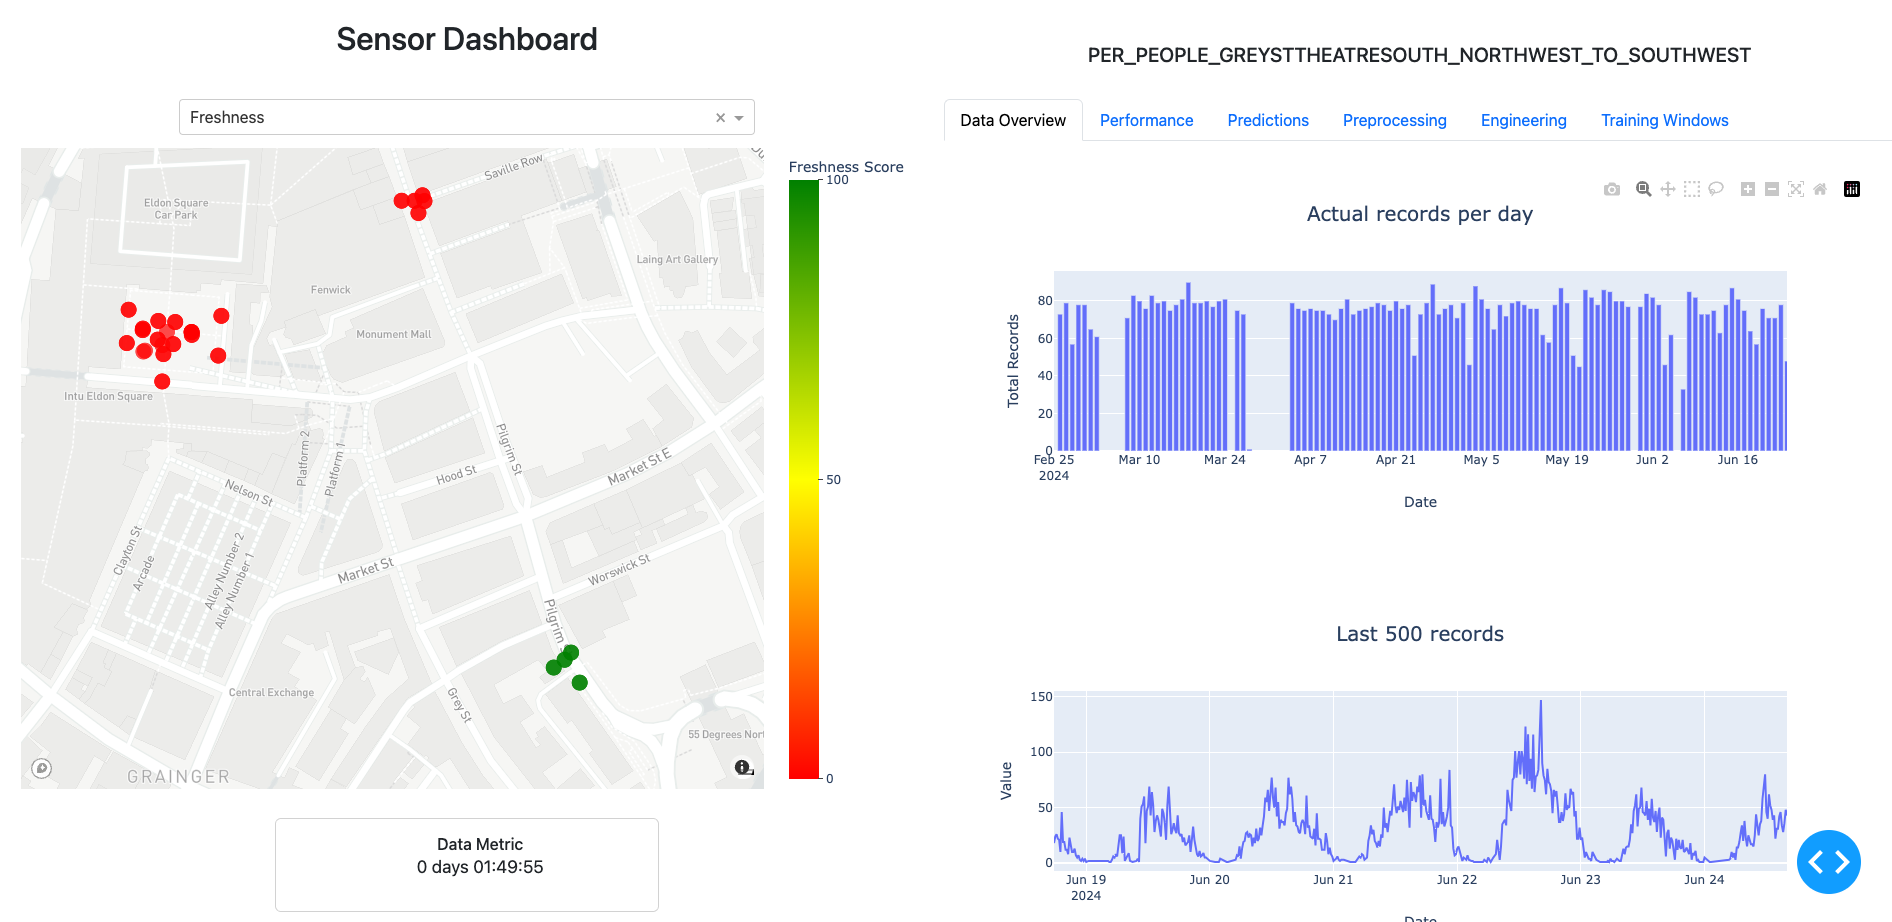
\includegraphics[scale=0.25]{figures/sensor_map_a.png}
    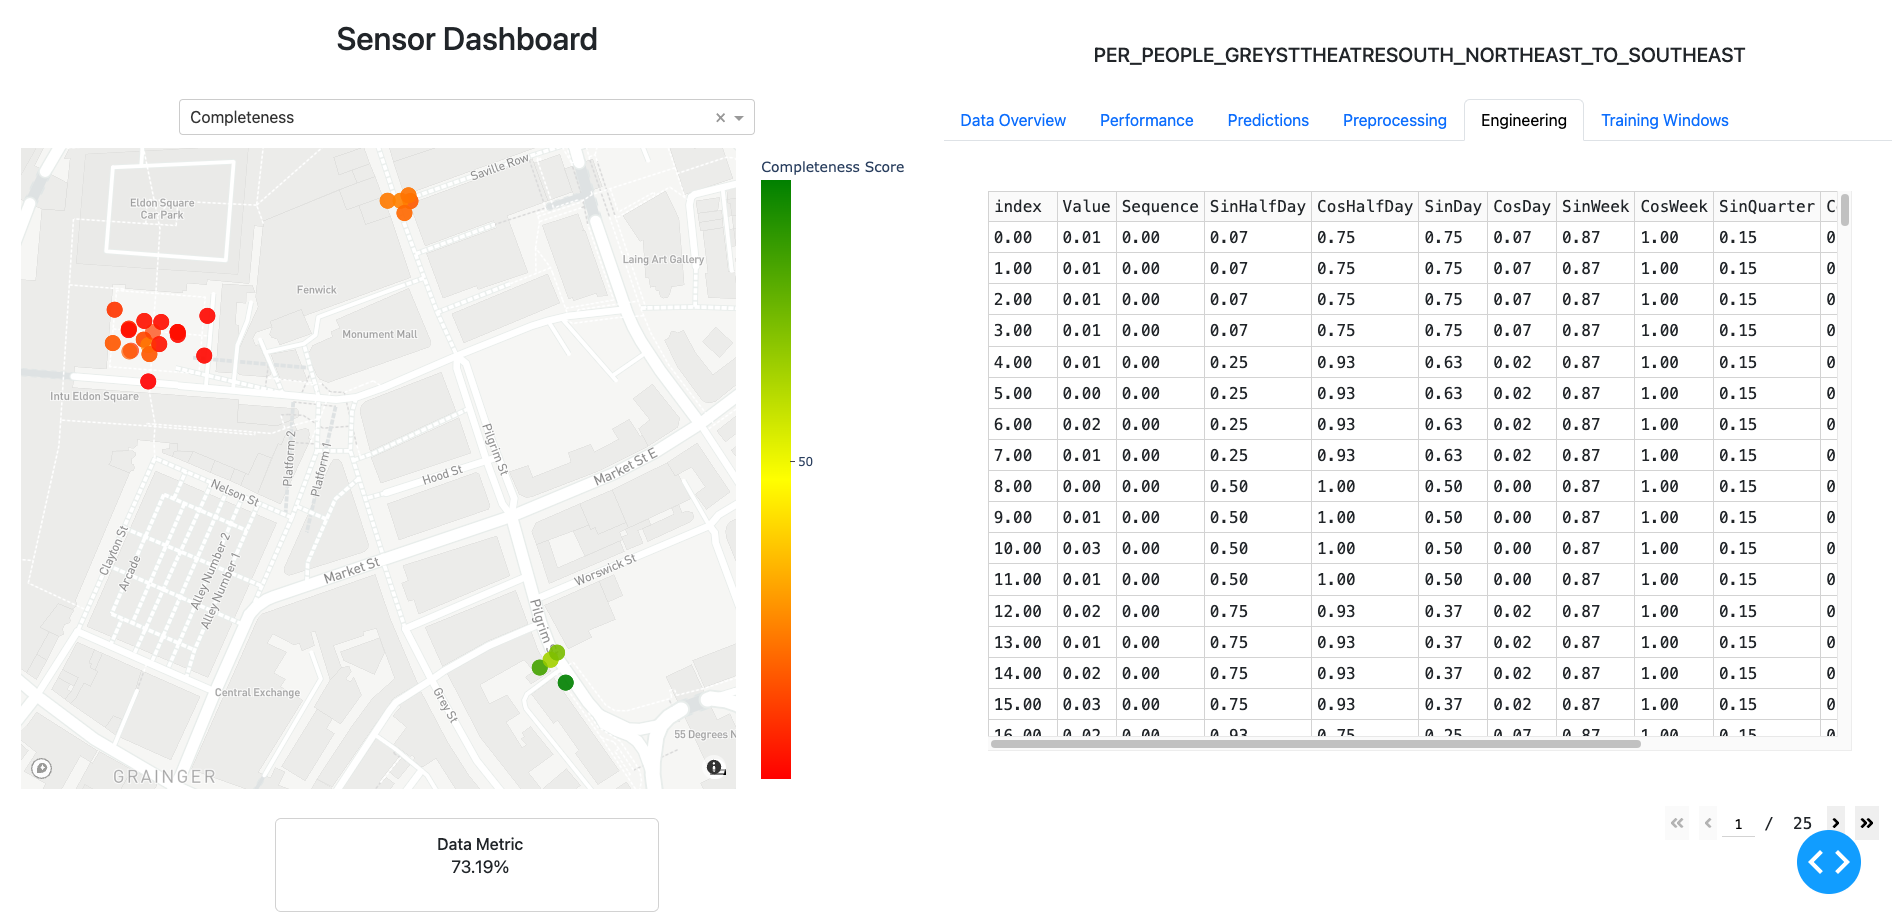
\includegraphics[scale=0.25]{figures/sensor_map_b.png}
    \caption{Dashboard}
    \label{fig:dashboard}
\end{figure}

\subsection{Literature Review}

The first draft of my literature is available \href{https://carrowmw.github.io/latex-documents/}{here} along with this document. As part of a skills development exercise, I have been using GitHub to host and manage the literature review (and other \LaTeX{} documents), developing a pdf viewer using JavaScript, and building in commenting functionality using \href{https://web.hypothes.is/}{hypothesis.is} to enable concurrent feedback from both supervisors. The literature review is currently undergoing feedback from my supervisors and will be revised accordingly. The literature review is focused primarily on quality-aware data streams specifically in the context of wireless sensor networks for smart cities. The case-study that is being used in this research is the pedestrian counting system developed by the Urban Observatory and Newcastle upon Tyne. The literature review has been structured to cover the following areas:

\begin{enumerate}
    \setlength{\itemindent}{3cm}
    \raggedright
    \item \textit{Data Quality Dimensions and Metrics}
    \item \textit{Data Quality Assessment}
    \item \textit{Data Quality Detection and Monitoring}
    \item \textit{Data Quality Management and Improvement}
    \item \textit{Data Quality Prediction and Proactive Approaches}
    \item \textit{Challenges and Future Directions}
\end{enumerate}
